\documentclass[11pt]{article}
\usepackage{color}
\usepackage{graphicx}
\usepackage{amsmath,amsthm,amssymb,multirow,paralist}
\usepackage[margin=0.8in]{geometry}
\usepackage{hyperref}

\begin{document}

\begin{center}
{\Large \textbf{COM S 573: Machine Learning}\\Homework \#5}\\

\linethickness{1mm}\line(1,0){498}

\begin{enumerate}
\item Please put required code files and report into a
compressed file ``HW\#\_FirstName\_LastName.zip''
\item Unlimited number of submissions are
allowed on Canvas and the latest one will be graded.
\item {\color{red} No later submission is accepted.}
\item Please read and follow submission instructions. No exception
will be made to accommodate incorrectly submitted files/reports.
\item All students are required to typeset their reports using
latex. Overleaf
(\url{https://www.overleaf.com/learn/latex/Tutorials}) can be a
good start.
\end{enumerate}

\linethickness{1mm}\line(1,0){498}

\end{center}

%%%%%%%%%%%%%%%%%%%%%%%%%%%%%%%%%%%%%%%%%%%%%%%%%%%%%%%%%%%%%%%%%%%%%%%%%%%%%%%

%%%%%%%%%%%%%%%%%%%%%%%%%%%%%%%%%%%%%%%%%%%%%%%%%%%%%%%%%%%%%%%%%%%%%%%%%%%%%%%


\begin{enumerate}

    \item (15 points) Given the convolutional neural network block as below
    \begin{center}
        \vspace{-10pt}
        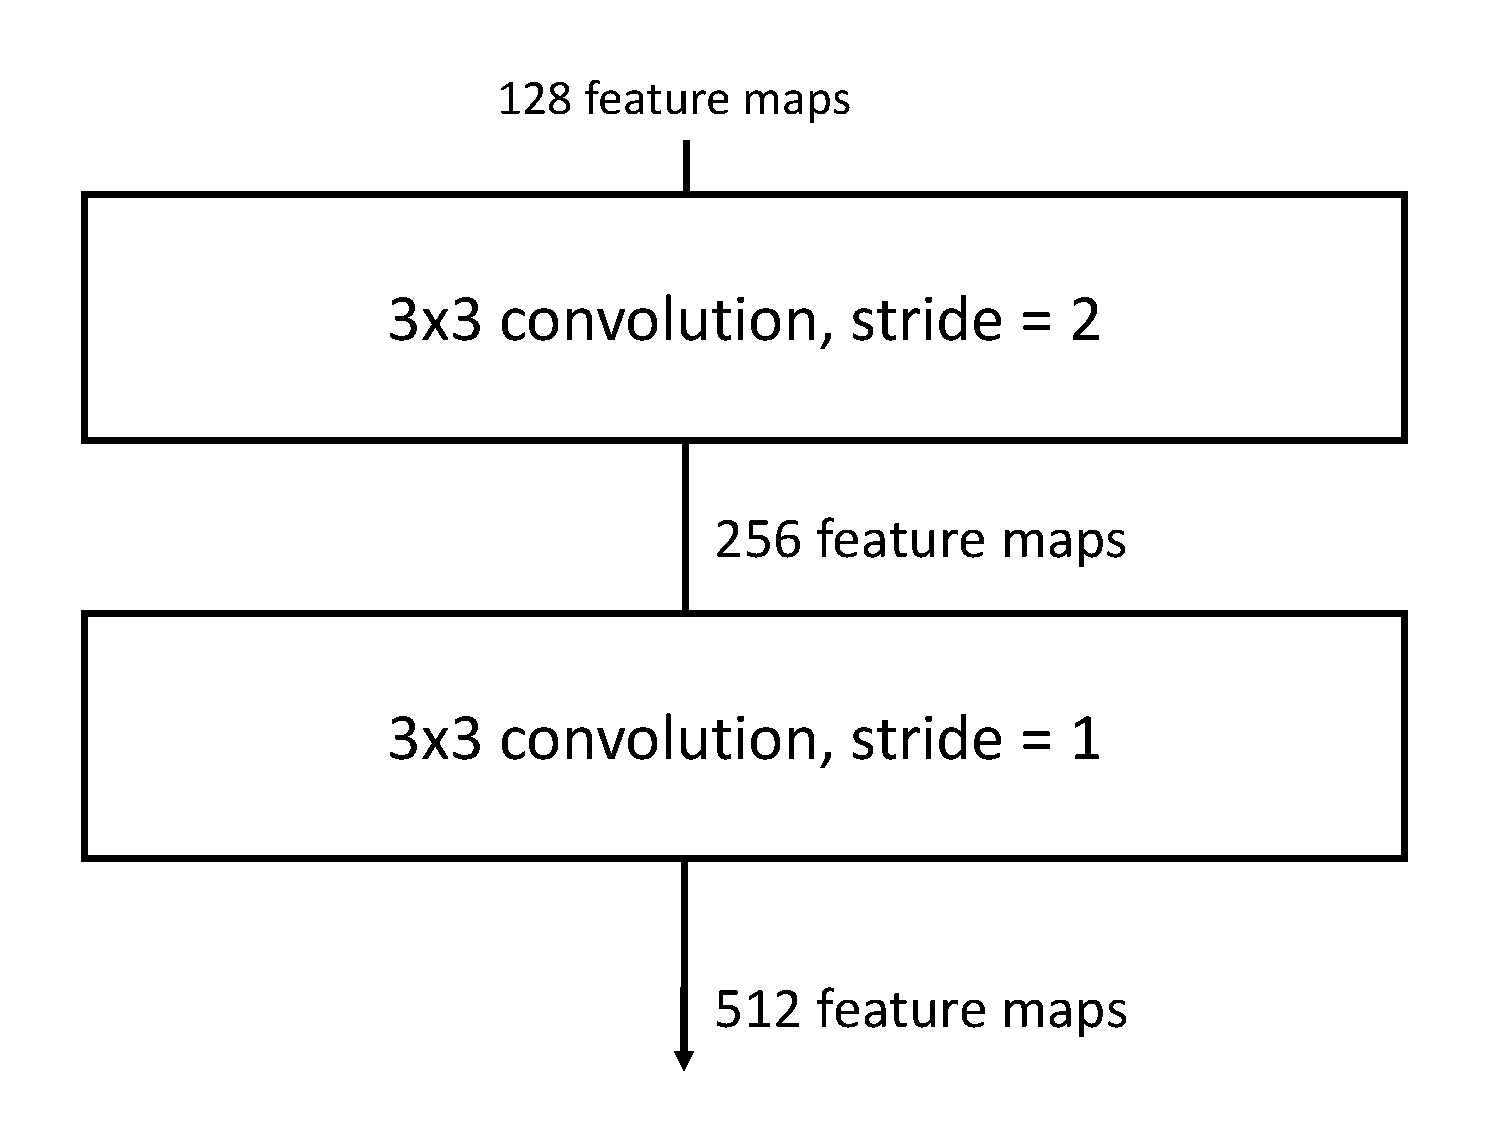
\includegraphics[width=0.45\textwidth]{FIG/cnnblock.pdf}
    \end{center}
    Given the input feature maps $\boldsymbol X \in
    \mathbb{R}^{64\times 64 \times 128}$, all convolutional
    layers perform zero-padding of $1$ on each side of $H$ and
    $W$ dimensions.
    \begin{enumerate}
    \item (5 points) What is the total number of parameters in
    the block (you can skip bias terms)?


    \item (5 points) What is the total number of multi-add
    operations in the block?


    \item (5 points) What is memory requirement change to store
    the input and output features of this block (Use percentage)?
    \end{enumerate}

    
    \item (20 points) Using batch normalization in neural networks requires computing
    the mean and variance of a tensor. Suppose a batch normalization
    layer takes vectors $z_1,z_2,\cdots,z_m$ as input, where $m$ is the
    mini-batch size. It computes $\hat z_1,\hat z_2,\cdots,\hat z_m$
    according to $$\hat z_i=\frac{z_i-\mu}{\sqrt{\sigma^2+\epsilon}}$$
    where $$\mu=\frac{1}{m}\sum_{i=1}^m
    z_i,\,\,\,\sigma^2=\frac{1}{m}\sum_{i=1}^m(z_i-\mu)^2.$$ It then
    applies a second transformation to obtain $\tilde z_1,\tilde
    z_2,\cdots,\tilde z_m$ using learned parameters $\gamma$ and $\beta$
    as $$\tilde z_i=\gamma \hat z_i+\beta.$$ In this question, you can
    assume that $\epsilon=0$.
    
    \begin{enumerate}
    \item (5 points) You forward-propagate a mini-batch of $m=4$ examples in your
    network. Suppose you are at a batch normalization layer, where the
    immediately previous layer is a fully connected layer with $3$
    units. Therefore, the input to this batch normalization layer can be
    represented as the below matrix:
    $$\begin{bmatrix}
    12&14&14&12\\
    0&10&10&0\\
    -5&5&5&-5
    \end{bmatrix}$$ What are $\hat z_i$? Please express your answer in a
    $3\times 4$ matrix.
    
    
    \item (5 points) Continue with the above setting. Suppose
    $\gamma=(1,1,1)$, and $\beta=(0,-10,10)$. What are $\tilde
    z_i$? Please express your answer in a $3\times 4$ matrix.

    
    \item (5 points) Describe the differences of computations required for batch normalization
    during training and testing.
    
    
    \item (5 points) Describe how the batch size during testing affect testing
    results.
    
    \end{enumerate}
    
    \item (20 points) We investigate the back-propagation of the convolution
    using a simple example. In this problem, we focus on the
    convolution operation without any normalization and
    activation function. For simplicity, we consider the
    convolution in 1D cases. Given 1D inputs with a spatial size
    of $4$ and $2$ channels, \emph{i.e.},
    \begin{equation}
    X=
    \begin{bmatrix}
    x_{11} & x_{12} & x_{13} & x_{14} \\
    x_{21} & x_{22} & x_{23} & x_{24}
    \end{bmatrix}
    \in \mathbb{R}^{2 \times 4},
    \end{equation}
    we perform a 1D convolution with a kernel size of $3$ to
    produce output $Y$ with $2$ channels. No padding is involved.
    It is easy to see
    \begin{equation}
    Y=
    \begin{bmatrix}
    y_{11} & y_{12} \\
    y_{21} & y_{22}
    \end{bmatrix}
    \in \mathbb{R}^{2 \times 2},
    \end{equation}
    where each row corresponds to a channel. There are 12
    training parameters involved in this convolution, forming 4
    different kernels of size $3$:
    \begin{equation}
    W^{ij} = [w^{ij}_1, w^{ij}_2, w^{ij}_3], i=1,2, j=1,2,
    \end{equation}
    where $W^{ij}$ scans the $i$-th channel of inputs and
    contributes to the $j$-th channel of outputs.


    \begin{enumerate}
    \item (5 points) Now we flatten $X$ and $Y$ to vectors as
    \begin{eqnarray}
    &&\tilde X = [x_{11}, x_{12}, x_{13}, x_{14} , x_{21}, x_{22}, x_{23}, x_{24}]^T \nonumber \\
    &&\tilde Y = [y_{11}, y_{12}, y_{21}, y_{22}]^T \nonumber
    \end{eqnarray}
    Please write the convolution in the form of fully connected
    layer as $\tilde Y=A\tilde X$ using the notations above. You
    can assume there is no bias term.\\Hint: Note that we
    discussed how to view convolution layers as fully connected
    layers in the case of single input and output feature maps.
    This example asks you to extend that to the case of multiple
    input and output feature maps.


    \item (5 points) Next, for the back-propagation, assume we've
    already computed the gradients of loss $L$ with respect to
    $\tilde Y$:
    \begin{equation}
    \frac{\partial L}{\partial \tilde Y}=\left [\frac{\partial L}{\partial y_{11}}, \frac{\partial L}{\partial y_{12}}, \frac{\partial L}{\partial y_{21}}, \frac{\partial L}{\partial y_{22}} \right ]^T,
    \end{equation}
    Please write the back-propagation step of the convolution in
    the form of $\frac{\partial L}{\partial \tilde
    X}=B\frac{\partial L}{\partial \tilde Y}.$ Explain the
    relationship between $A$ and $B$.


    \item (10 points) While the forward propagation of the
    convolution on $X$ to $Y$ could be written into $\tilde
    Y=A\tilde X$, could you figure out whether $\frac{\partial
    L}{\partial \tilde X}=B\frac{\partial L}{\partial \tilde Y}$
    also corresponds to a convolution on $\frac{\partial
    L}{\partial Y}$ to $\frac{\partial L}{\partial X}$? If yes,
    write down the kernels for this convolution. If no, explain
    why.


    \end{enumerate}
    
    
    \item (45 points) \textbf{LeNet for Image Recognition:} In
    this coding assignment, you will need to complete the
    implementation of LeNet (LeCun Network) using PyTorch and
    apply the LeNet to the image recognition task on Cifar-10
    (10-classes classification). You will need to install the
    python packages ``tqdm'' and ``pytorch''. Please read the
    installation guides of PyTorch here
    (https://pytorch.org/get-started/locally/). You are expected
    to implement your solution based on the given codes. The only
    file you need to modify is the ``solution.py'' file. You can
    test your solution by running the ``main.py'' file.
    
    \begin{enumerate}
    \item (25 points) Complete the class \emph{\textbf{LeNet()}}.
    In particular, define operations in function
    \emph{\textbf{\_\_init\_\_()}} and use them in function
    \emph{\textbf{forward()}}. The input of
    \emph{\textbf{forward()}} is an image. The paper for LeNet
    can be found here
    (http://yann.lecun.com/exdb/publis/pdf/lecun-01a.pdf)
    
    The network architecture is shown in the figure below.
    \begin{center}
    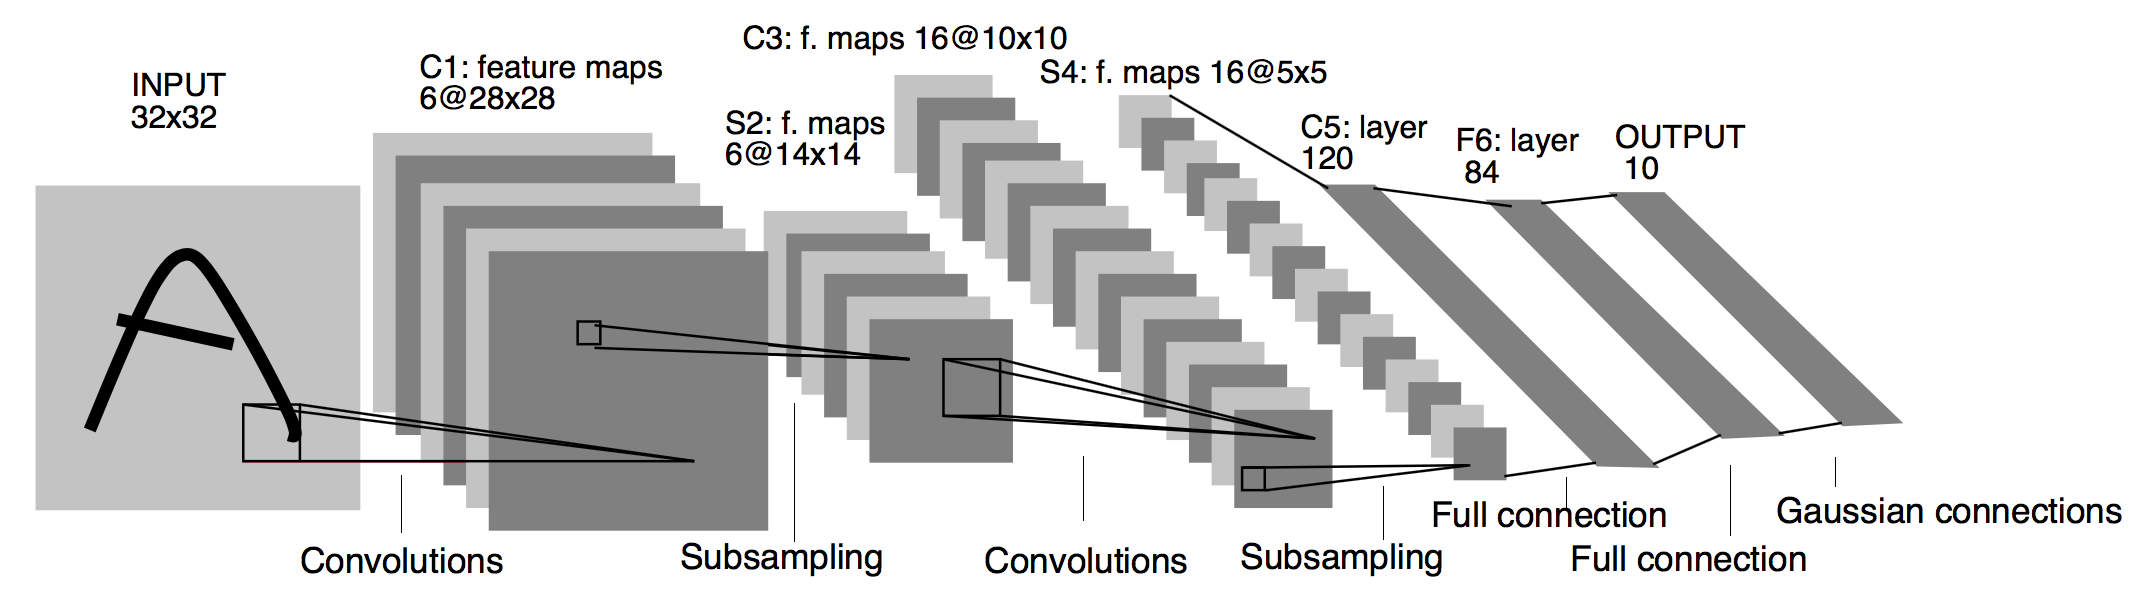
\includegraphics[scale=0.18]{FIG/LeNet.png}
    \end{center}
    
    The sub-sampling is implemented by using the max pooling. And
    the kernel size for all the convolutional layers are $5\times
    5$. Please use \emph{\textbf{ReLU}} function to activate the
    outputs of convolutional layers and the first two
    fully-connected layers. The sequential layers are:
    \begin{align*}
    &\text{Inputs} \to \\
    &\text{Convolution (6 out channels)} \to \text{Max Pooling} \to \\
    &\text{Convolution (16 out channels)}\to \text{Max Pooling}\to\\
    &\text{Reshape to vector}\to \text{Fully-connected (120 out units)}\to \\
    &\text{Fully-connected (84 out units)}\to \text{Outputs (n\_classes out units)}
    \end{align*}
    
    For this part, you are only allowed to use the APIs in
    \emph{\textbf{torch.nn}}. Please refer to the PyTorch API
    documents below for the usage of those APIs before you use
    them: \\
    https://pytorch.org/docs/stable/nn.html.

    Run the model by ``\emph{\textbf{python main.py}}'' and
    report the testing performance as well as a short analysis of
    the results.


    \item (10 points) Add batch normalization operations after
    each max pooling layer. Run the model by
    ``\emph{\textbf{python main.py}}'' and report the testing
    performance as well as a short analysis of the results.


    \item (10 points) Based on (b), add dropout operations with
    drop rate of 0.3 after the first two fully-connected layers.
    Run the model by ``\emph{\textbf{python main.py}}'' and
    report the testing performance as well as a short analysis of
    the results.

    
    \end{enumerate}
    
    \end{enumerate}

\end{document}
